% Preamble
\documentclass[11pt]{beamer}
% Add xcolor with dvipsnames to define structure colors
\usepackage[dvipsnames]{xcolor}
\mode<presentation>{
  \usetheme{Madrid}
  \usecolortheme[named=Periwinkle]{structure}
  \useoutertheme{shadow}
  \setbeamertemplate{navigation symbols}{}
  \setbeamertemplate{headline}{}
}
\usepackage[italian]{babel}
\usepackage[utf8]{inputenc}
\usepackage[T1]{fontenc}
\usepackage{graphicx}
\hypersetup{
  pdftitle={Performance Analysis for Projection-Correction Methods in Motion Deblurring Problems},
  pdfauthor={Sara Casadio, Enrico Ferraiolo, Giovanni Savoca}
}

% Title and Author
\title[Progetto]{Performance Analysis for Projection-Correction Methods in Motion Deblurring Problems}
\author[Autore]{Sara Casadio, Enrico Ferraiolo, Giovanni Savoca}
\institute[Istituzione]{%
  Alma Mater Studiorum - Università di Bologna \\
  Corso di Laurea in Informatica
}
\date{\today}

\begin{document}

% Title Frame
\begin{frame}
  \titlepage
\end{frame}

% Section 1
\section{Descrizione del problema}
\subsection{Problem Description}
\begin{frame}{Problem Description}
  \begin{itemize}
    \item The project analyzes the performance of two \textbf{Projection-Correction} algorithms for reconstructing medical images affected by \textbf{motion blur}.
    \item The studied algorithms are:
    \begin{itemize}
      \item \textbf{Diffusion Posterior Sampling (DPS)}
      \item \textbf{Regularization by Denoising with Diffusion (RED-Diff)}
    \end{itemize}
    \item Both methods are based on \textbf{pre-trained diffusion models}.
    \item Objective: evaluate the effectiveness of these methods in recovering degraded images.
  \end{itemize}
\end{frame}

% Section 2
\section{Approccio di risoluzione con dps e rediff + modello diffusivo}
\subsection{Approach to the Problem}
\begin{frame}{Approach to the Problem}
  \begin{itemize}
    \item \textbf{Objective}: Analyze the performance of \textit{Projection-Correction} methods \textbf{DPS} and \textbf{RED-Diff} for motion blur removal on medical images
    \item \textbf{Phase 1}: Dataset preprocessing (128x128)
    \item \textbf{Phase 2}: Data augmentation to increase dataset diversity
    \item \textbf{Phase 3}: Training a DDIM diffusion model on medical data
    \item \textbf{Phase 4}: Simulation of motion blur and its removal
    \item \textbf{Phase 5}: Implementation and comparison of \textit{Projection-Correction} methods: \textbf{DPS} and \textbf{RED-Diff}
    \item \textbf{Phase 6}: Quantitative evaluation of performance using metrics such as \textbf{PSNR} and \textbf{SSIM}
  \end{itemize}
\end{frame}

% Section 3
\section{Dataset} %Preprocessing del dataset (128*128) + dataset aumentato 
\subsection{Mayo Clinic CT Dataset}

\begin{frame}{Mayo Clinic CT Dataset}
  \begin{itemize}
    \item Released by the \textbf{Mayo Clinic} for research purposes.
    \item Contains chest \textbf{Computed Tomography (CT)} scans.
    \item Images are in \textbf{grayscale (black and white)} format.
    \item Focus on \textbf{lung nodules} and early detection of \textbf{lung cancer}.
    \item Widely used in machine learning and AI medical imaging research.
  \end{itemize}
  \vspace{0.5cm}
  \begin{center}
    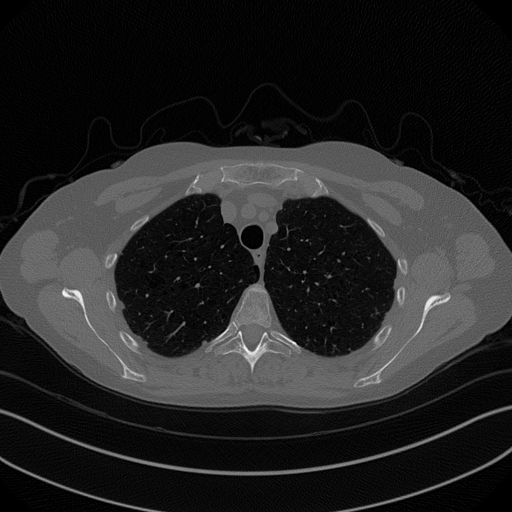
\includegraphics[width=0.25\linewidth]{media/2.png}
    \hspace{0.3cm}
    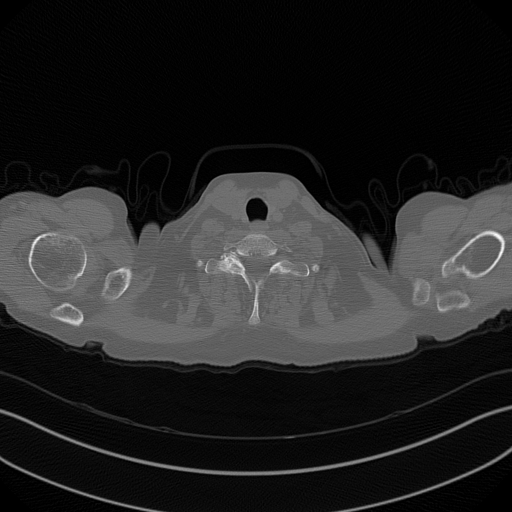
\includegraphics[width=0.25\linewidth]{media/3.png}
    \hspace{0.3cm}
    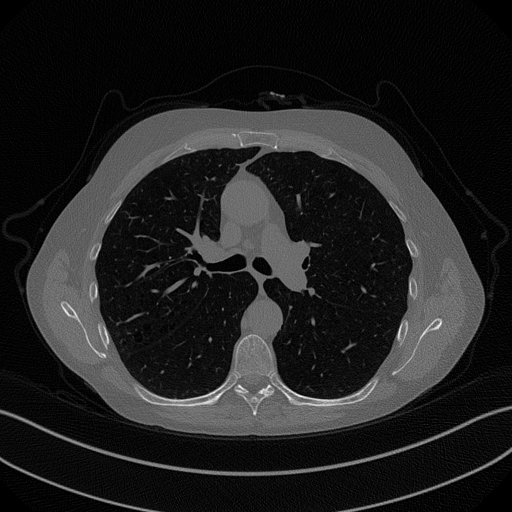
\includegraphics[width=0.25\linewidth]{media/100.png}
  \end{center}
\end{frame}

\begin{frame}{Preprocessing and Augmentation}
  \begin{itemize}
    \item All CT images were preprocessed and resized to a fixed dimension of \textbf{128 × 128 pixels}.
    \item This standardization ensures consistency for input into deep learning models.
    \item The dataset was \textbf{augmented} to avoid overfitting and improve model generalization (detailed later).
  \end{itemize}
\end{frame}

% Section 4
\section{organizzazione della repository}
\subsection{Sottosezione 2.1}
\begin{frame}{Sottosezione 2.1}
  % Contenuto qui
\end{frame}

% Section 5
\section{architettura della rete diffusiva} 
\subsection{Sottosezione 2.1}
\begin{frame}{Sottosezione 2.1}
  % Contenuto qui
\end{frame}

% Section 6
\section{Training} %data augmentation + data loader + scheduler + torch.compite + grade scaler + cosineannealing + spiegaizone dello step di apprendimento della reta + per ogni epoca viene stampata una immagine per capire se la rete sta funzionando + spiegazione loss (come funziona) + salvataggio pesi + grafico loss
\subsection{Sottosezione 2.1}
\begin{frame}{Sottosezione 2.1}
  % Contenuto qui
\end{frame}

% Section 7
\section{Caricamento dei pesi (come funziona che non dobbiamo sempre allenare il modello e possiamo caricarli deìirettamente )} 
\subsection{Sottosezione 2.1}
\begin{frame}{Sottosezione 2.1}
  % Contenuto qui
\end{frame}

% Section 8
\section{codice dei due metodi} 
\subsection{Sottosezione 2.1}
\begin{frame}{Sottosezione 2.1}
  % Contenuto qui
\end{frame}

% Section 9
\section{codice immagine degradata} 
\subsection{Sottosezione 2.1}
\begin{frame}{Sottosezione 2.1}
  % Contenuto qui
\end{frame}

% Section 9
\section{risultati} 
\subsection{Sottosezione 2.1}
\begin{frame}{Sottosezione 2.1}
  % Contenuto qui
\end{frame}

% Conclusions
\section{Conclusioni}
\begin{frame}{Conclusioni}
  % Punti chiave
\end{frame}

% Thank You Frame
\begin{frame}
  \centering
  {\Huge Grazie per l'attenzione}
\end{frame}

\end{document}